\documentclass{article}
\usepackage[utf8]{inputenc}
\usepackage{graphicx}
\usepackage{epstopdf}
\usepackage{float}
\usepackage[margin=1.25in]{geometry}
\usepackage{amsmath}
\usepackage{amssymb}
\usepackage{color} 
\usepackage{fancyvrb} 
\title{Circuits Lab 6}
\author{Cory Dolphin and Noam Rubin}
\date{April 3, 2013}

\begin{document}

\maketitle

\section*{Current as a function of voltage}
% In your report, include a single plot showing I1, I2, I1−I2, and I1+I2, as a function of V1−V2 for all three values of V2 that you used. Do these current–voltage characteristics change significantly asV2 changes? 

\begin{figure}[H]
\centering
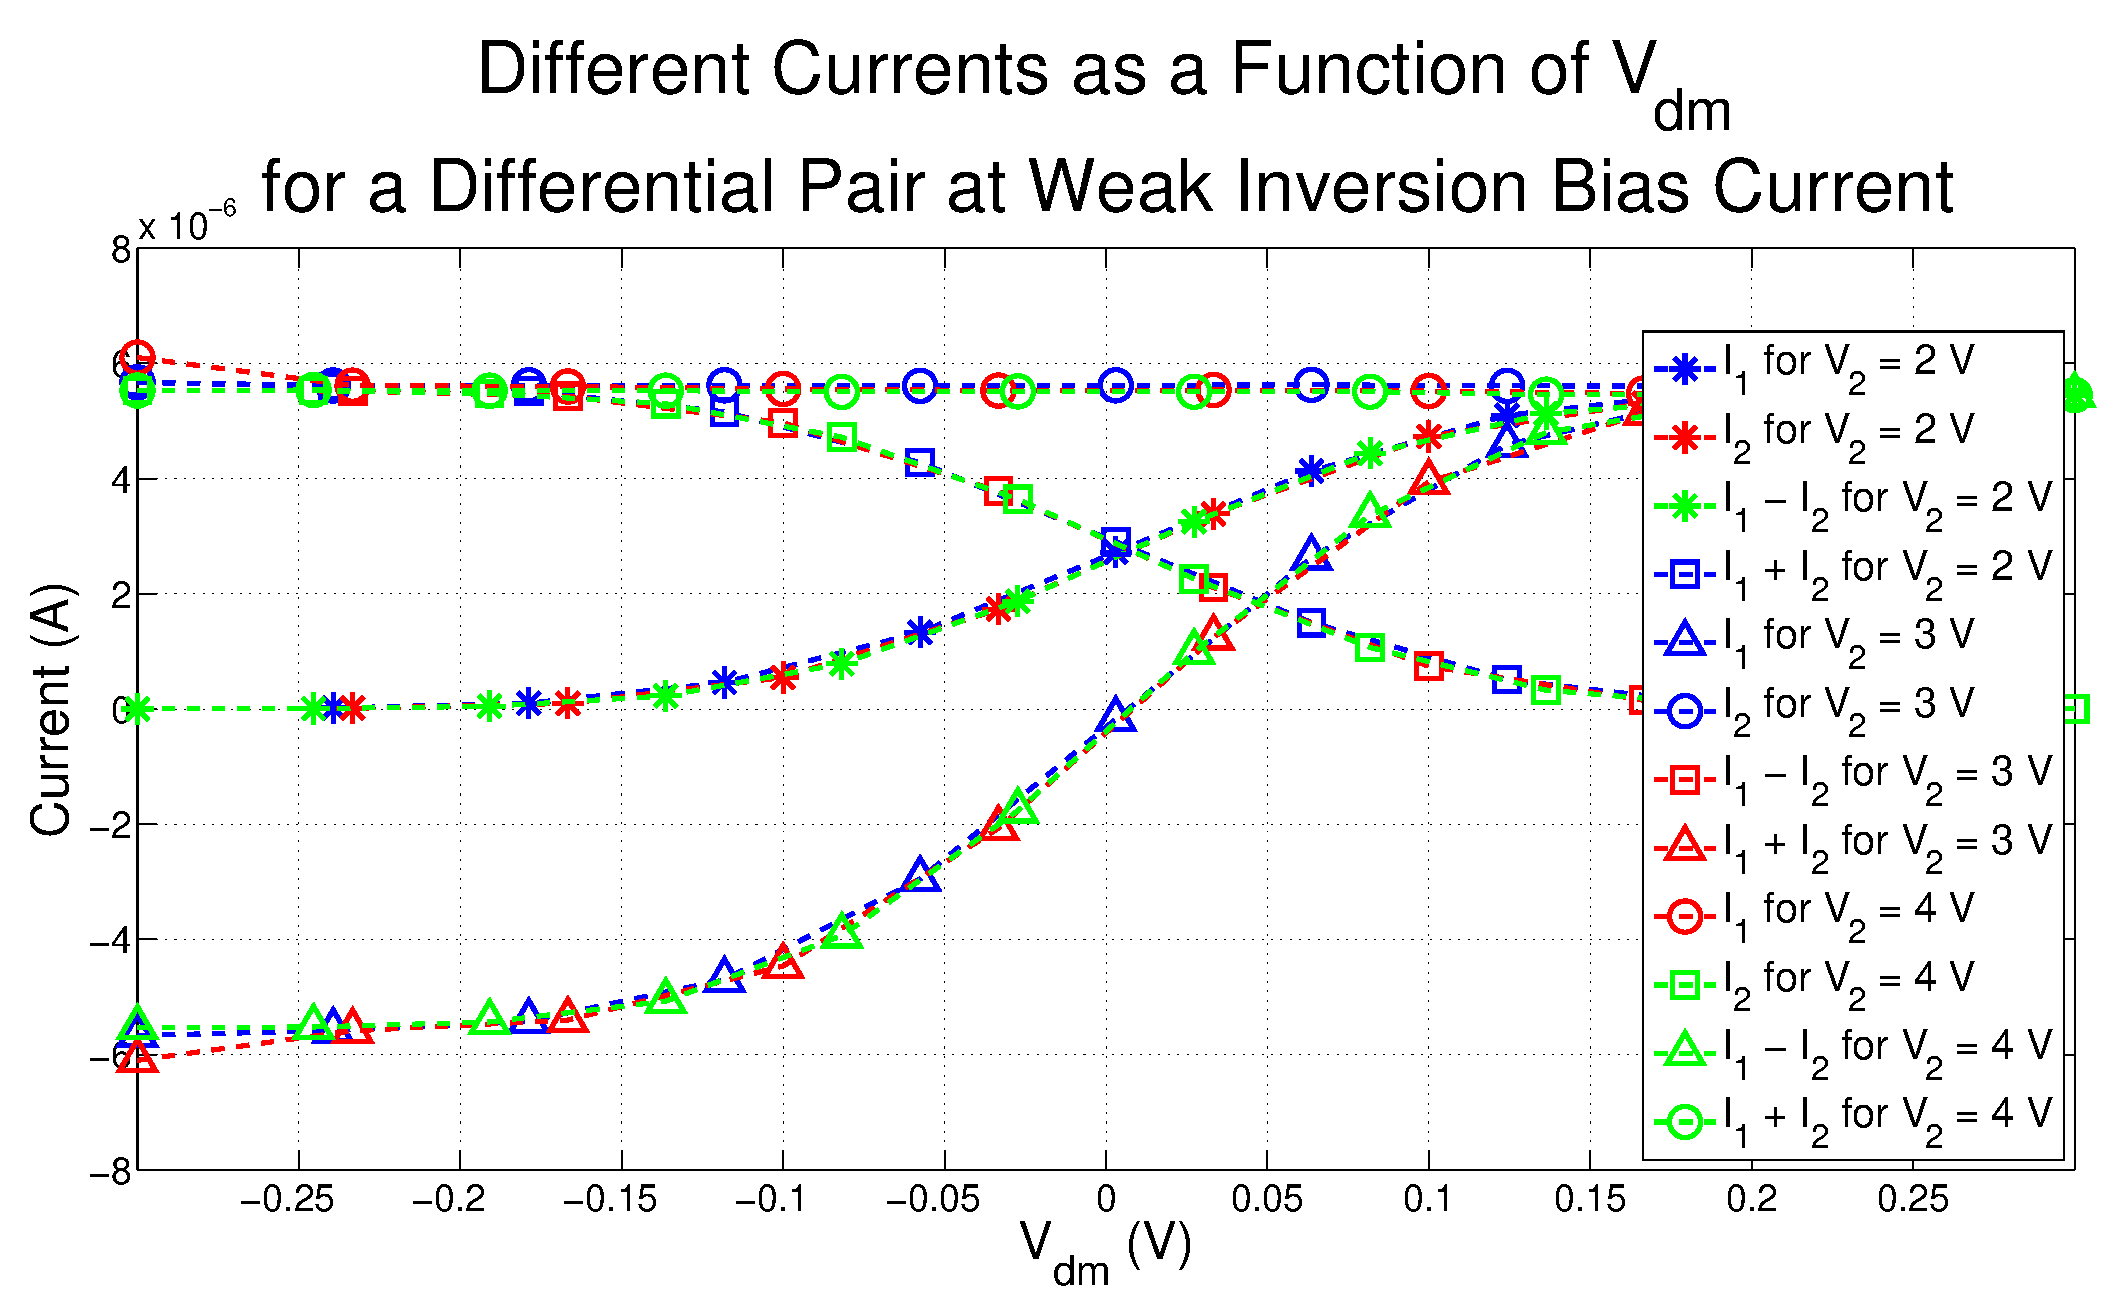
\includegraphics[width=\linewidth]{./Figures/AllCurrentsOneFigure}
\caption{Something descriptive. }
\label{fig:AllCurrentsOneFigure }
\end{figure}


\begin{figure}[H]
\centering
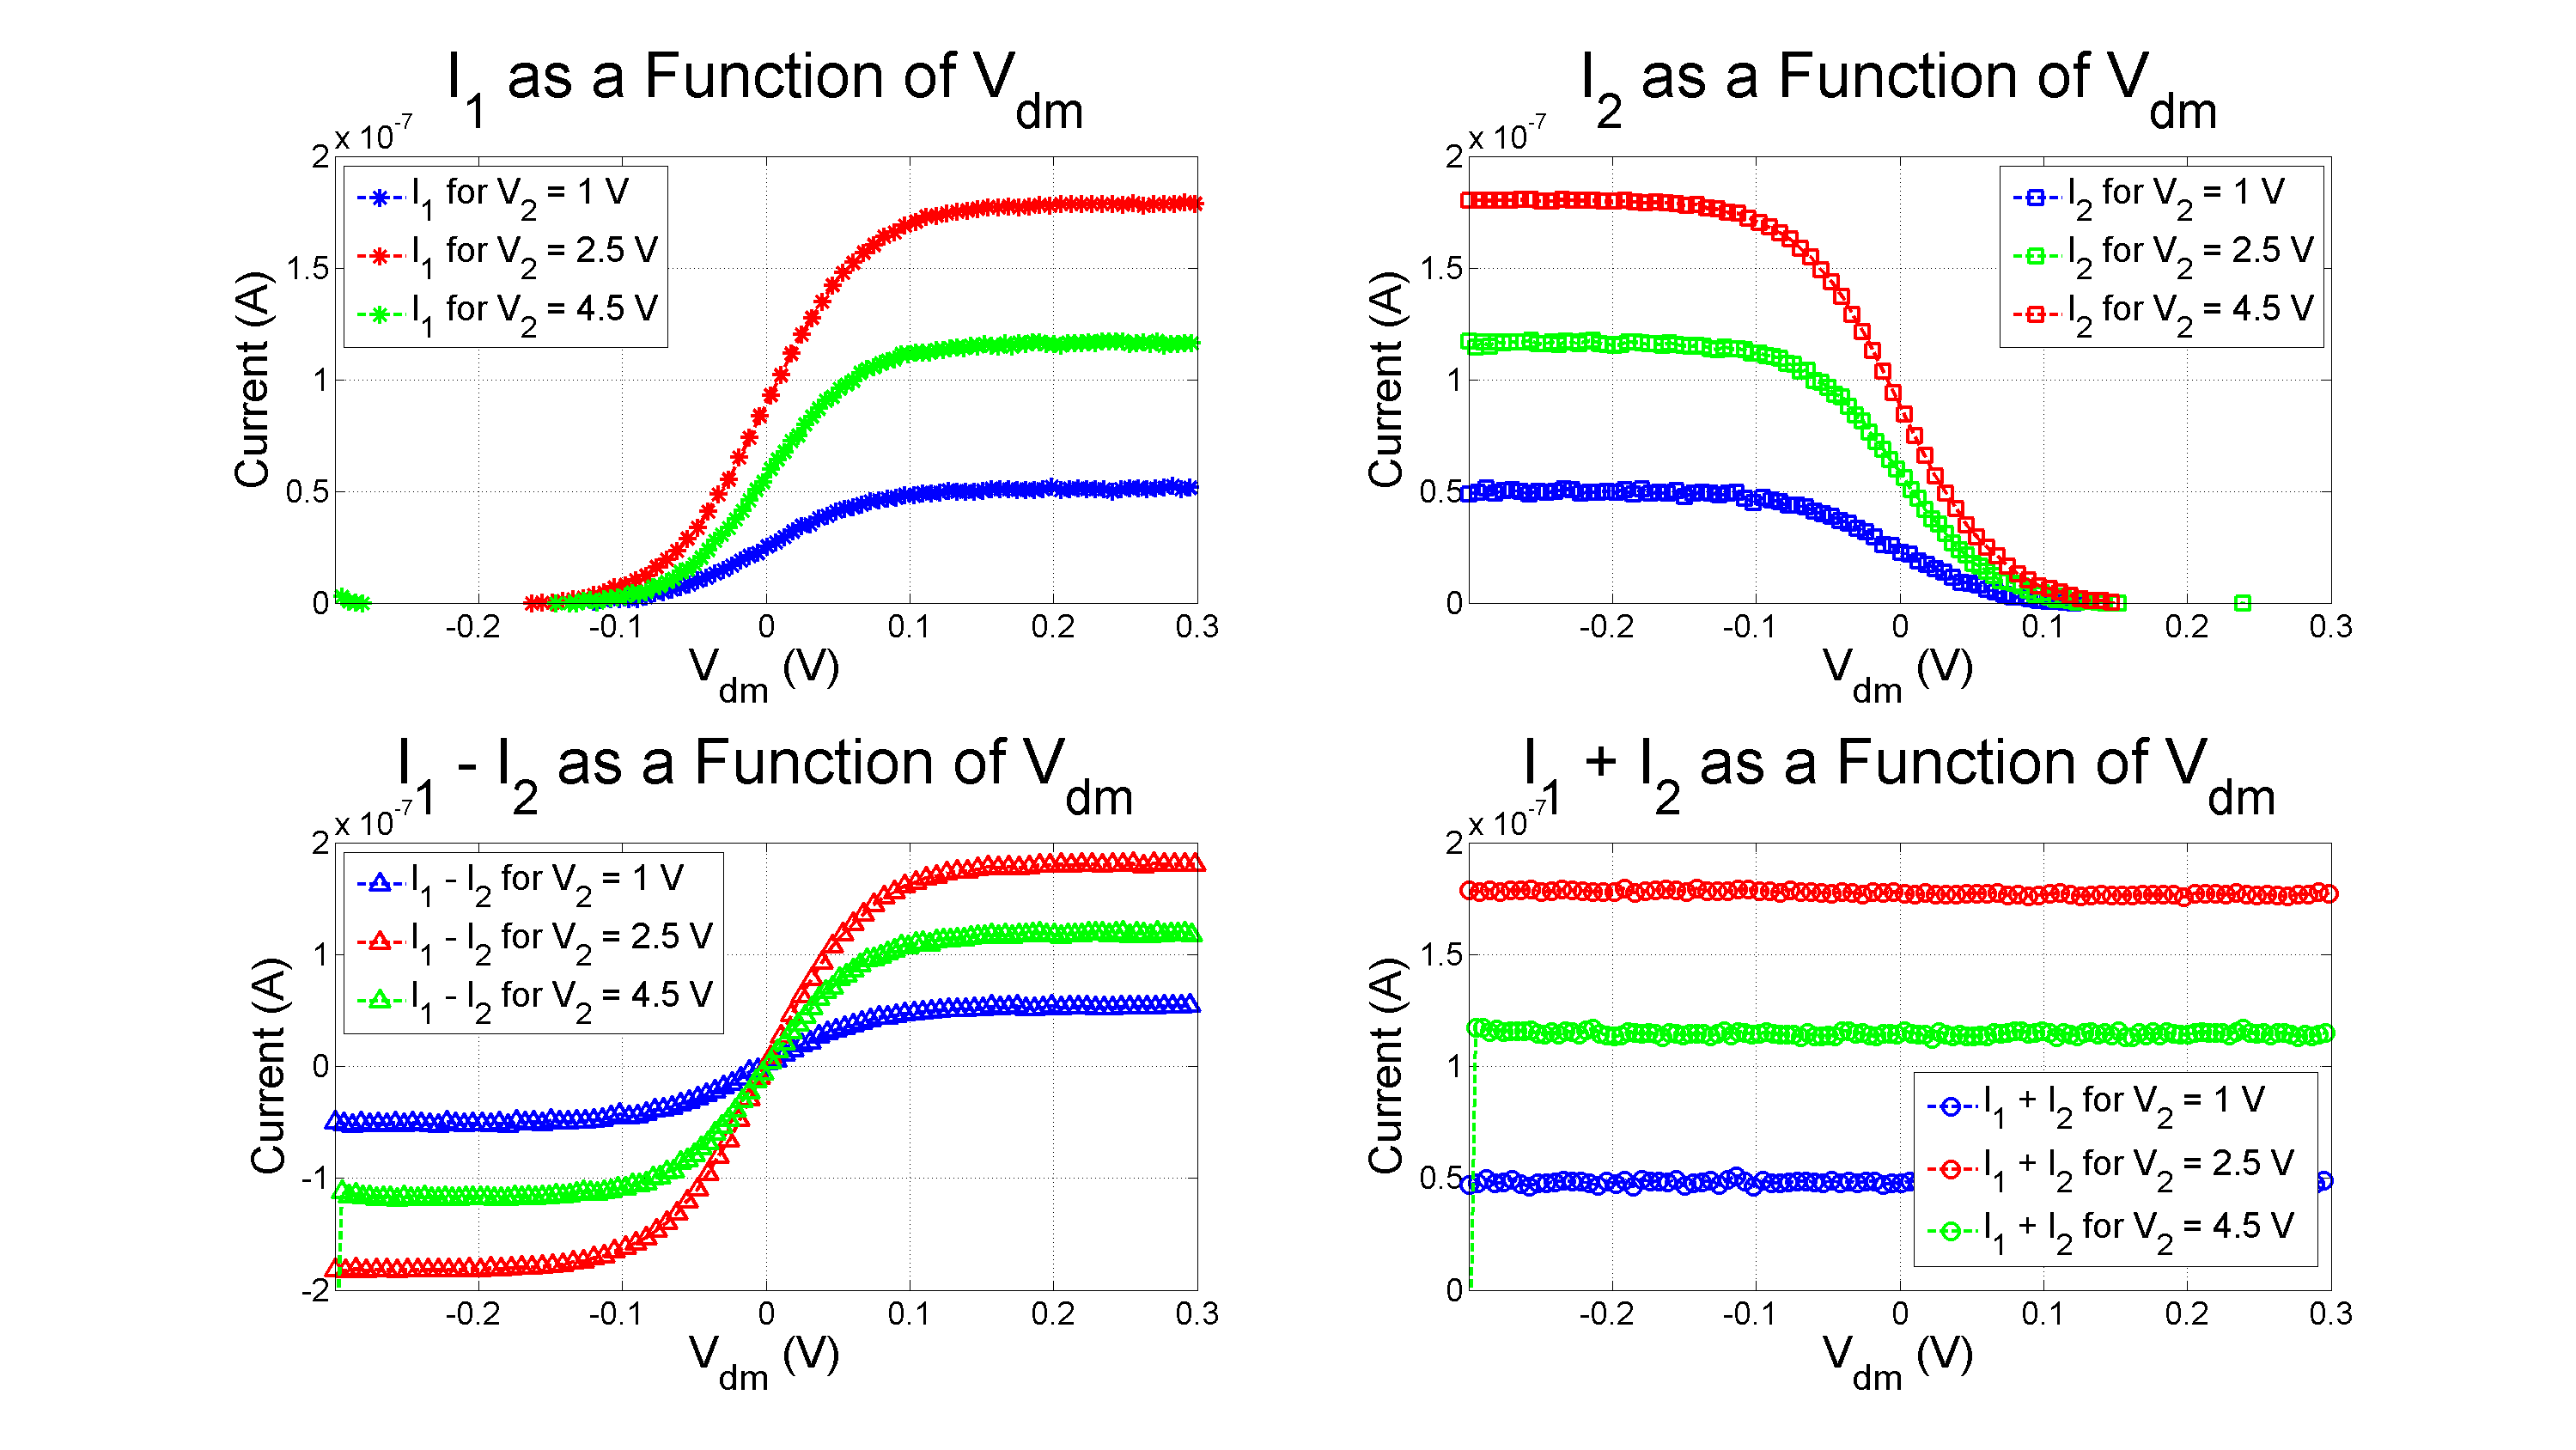
\includegraphics[width=\linewidth]{./Figures/AllCurrentsSubplot}
\caption{Something descriptive.}
\label{fig:AllCurrentsSubplot}
\end{figure}

\section*{Common-source Node voltage}
% Also include a plot showing the common-source node voltage, V , as a functionof V1−V2 for all three values of V2. How does the value of V change as V1 goes from below V2 to above it?

%NodeVoltageWeakInversion

\begin{figure}[H]
\centering
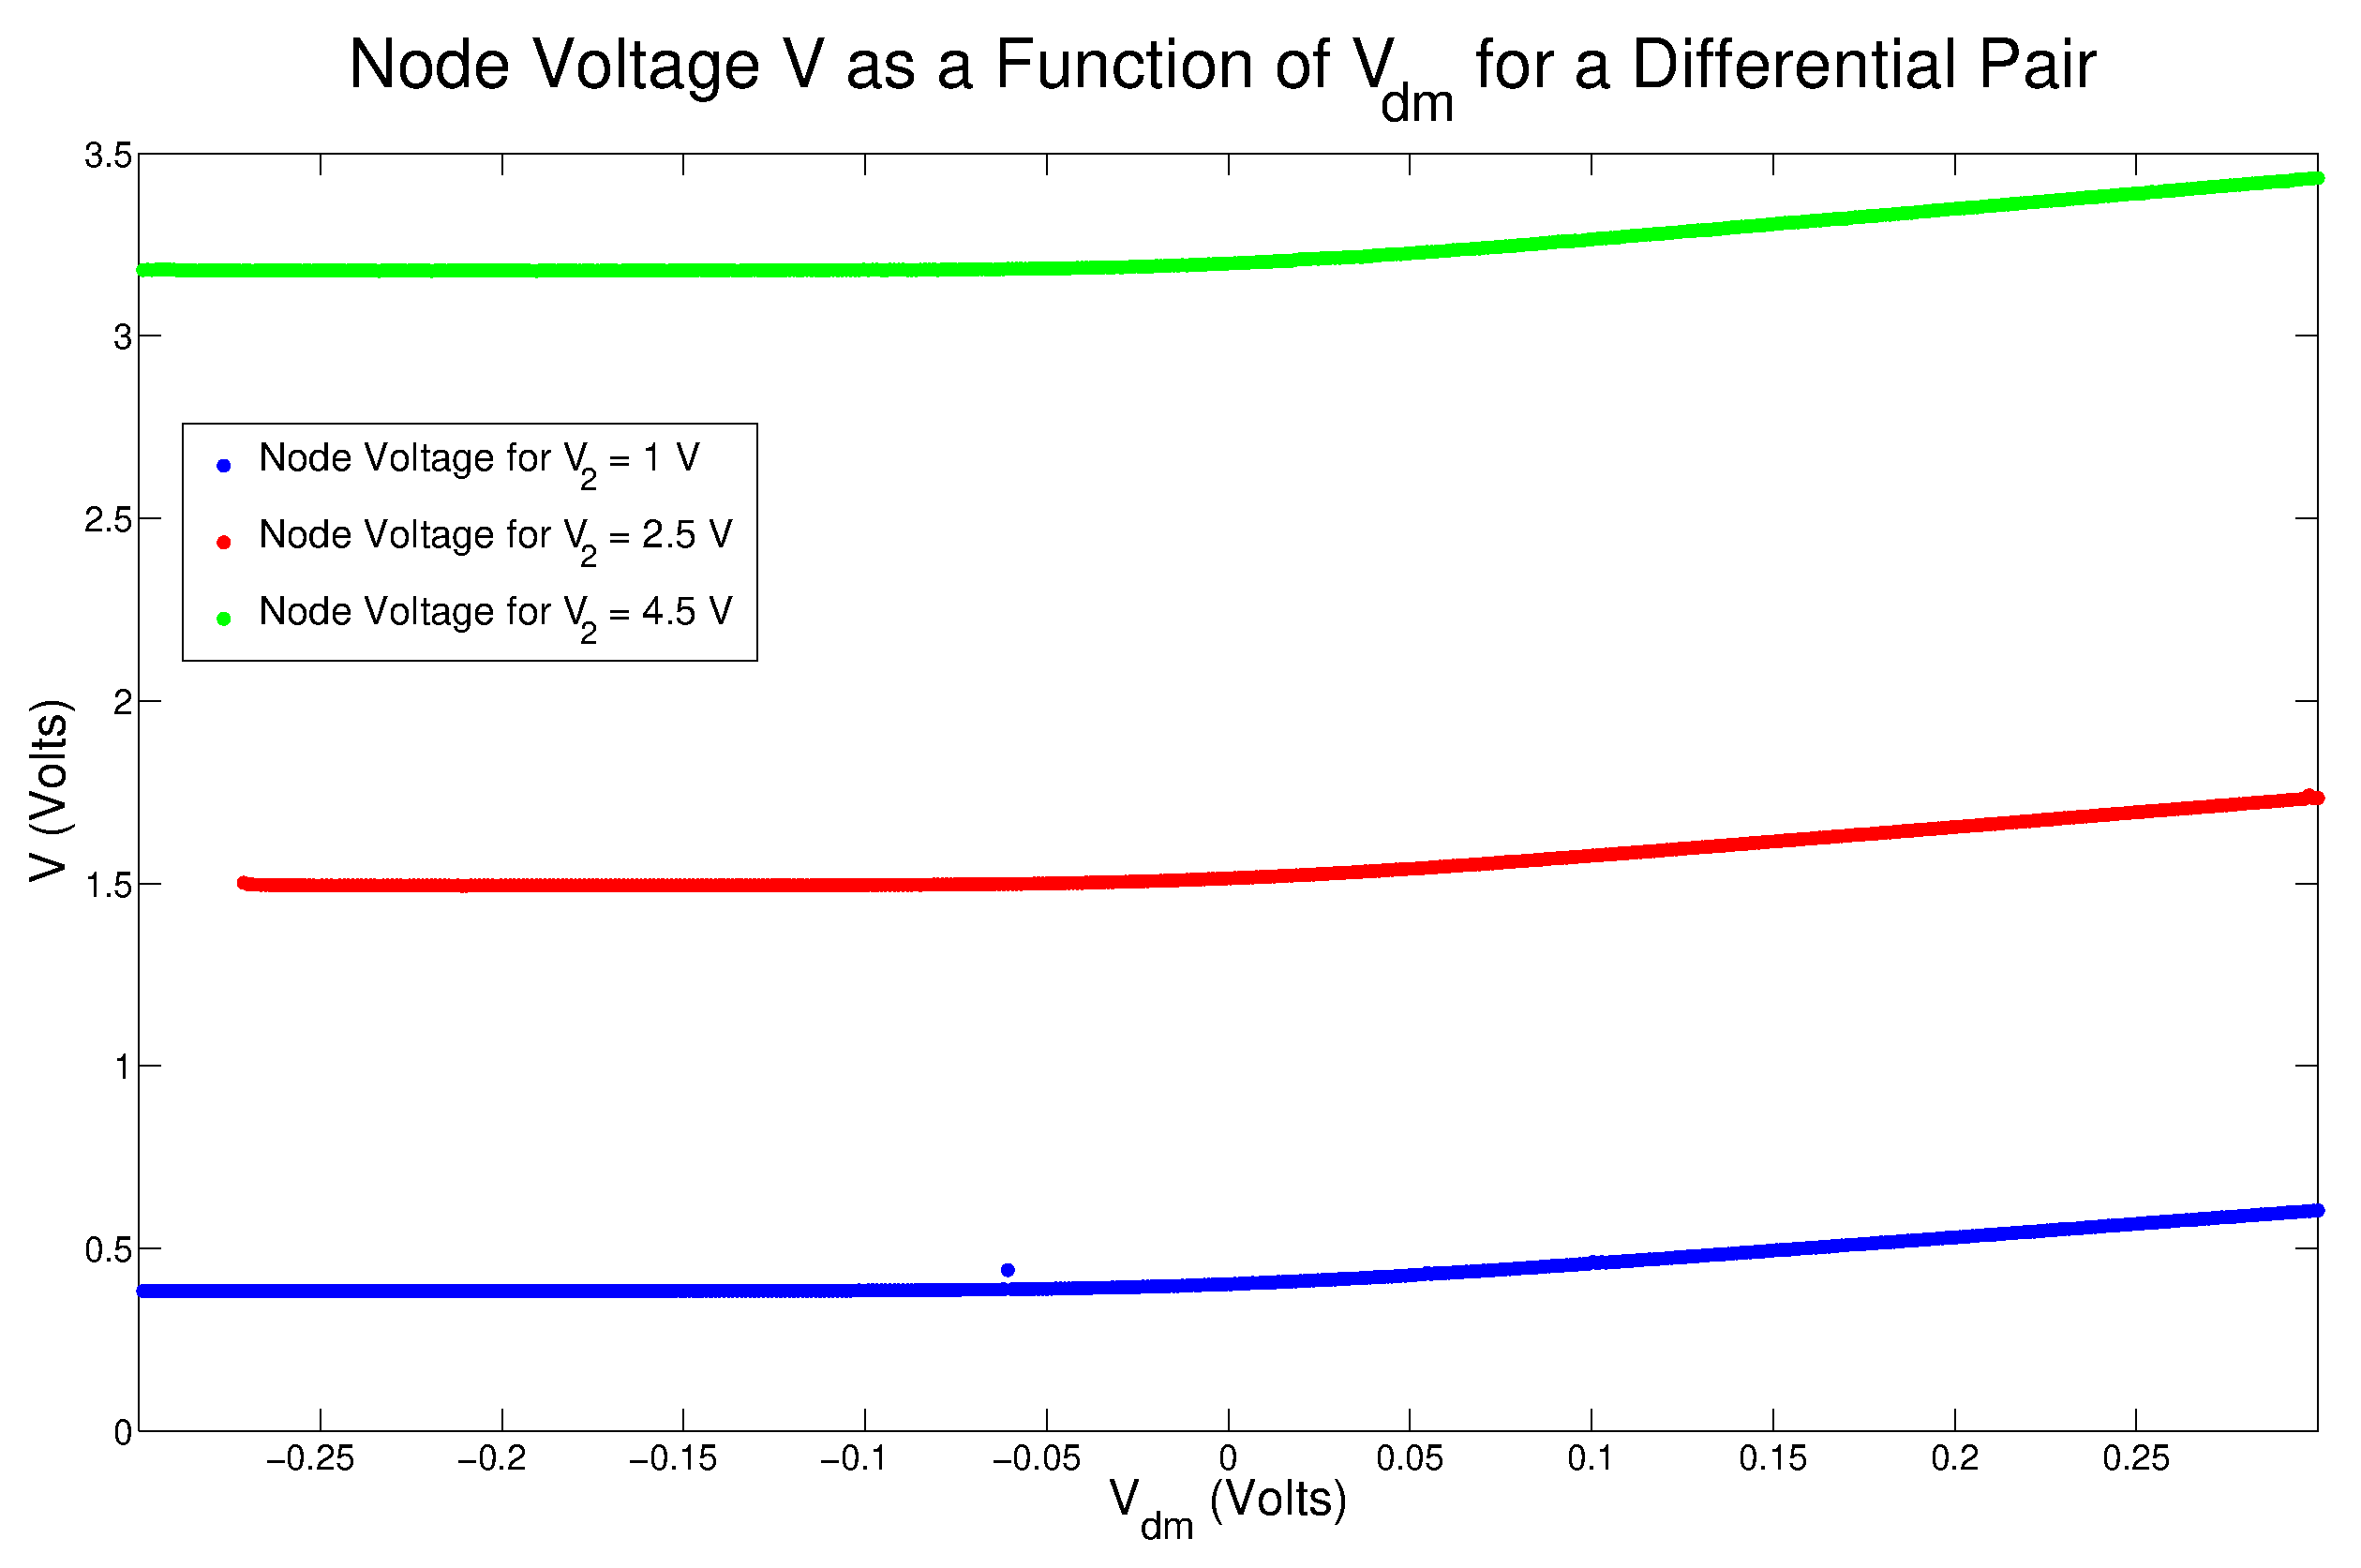
\includegraphics[width=\linewidth]{./Figures/NodeVoltageWeakInversion.eps}
\caption{The node voltage follows the larger voltage!!}
\label{fig:nodevoltageWI}
\end{figure}

% For each of the three values of V2 that you used, fit a straight line to the plot of I1−I2 asa function of V1− V2 around the region where V1~ V2 (i.e., where V1−V2~ 0). The slope of this line is approximately equal to the (incremental) differential-mode transconductancegain of the differential pair, which is formally given by ... Does the value of the differential-mode transconductance gain change significantly as V2 changes?

\begin{figure}[H]
\centering
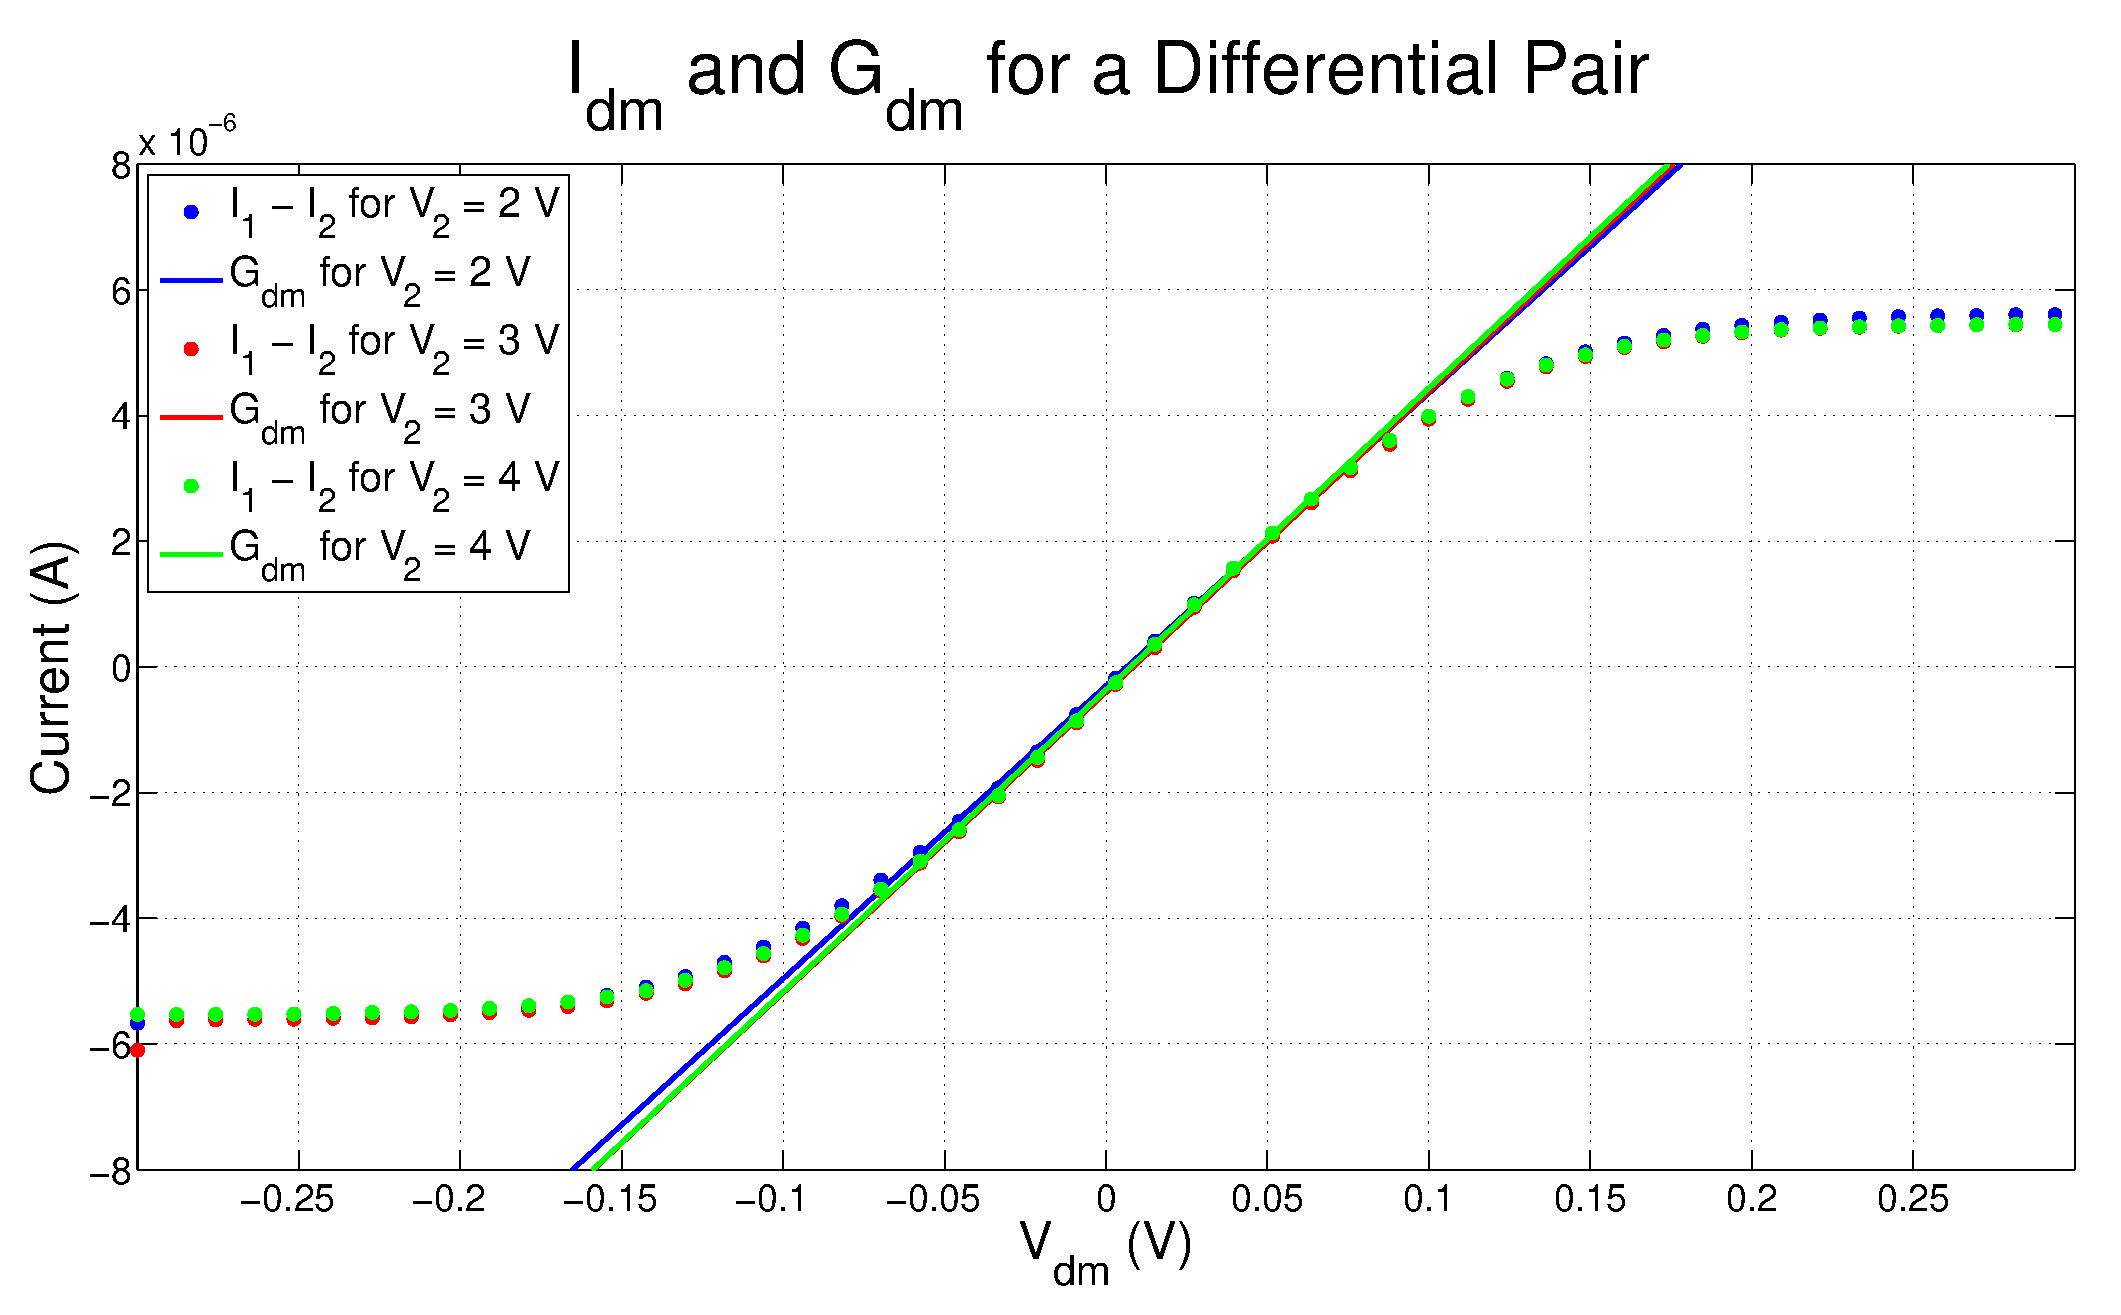
\includegraphics[width=\linewidth]{./Figures/Gdm.eps}
\caption{Gdm changes!!}
\label{fig:gdm}
\end{figure}

\begin{table}[h]
\begin{center}
    \begin{tabular}{ l | l  }
        V2 (Volts) & $G_{dm} (\Omega^{-1})$ \\
        \hline
        1 & $6.7086 \times 10^{-7}$ \\
        2.5 & $2.4470 \times 10^{-6}$ \\
        4.5 & $1.6894 \times 10^{-6}$ \\
        \label{tb:gdm}
    \end{tabular}
\end{center}
\end{table}


% Now, set the bias voltage, Vb, so that the bias current is above threshold. For a singlevalue of V2 that is far enough away from the power supply rail to keep the bias transistor saturated, perform these same measurements. You might want to increase slightly the rangeover which you sweep V1− V2 for these measurements. Make plot similar to the ones thatyou made for the lower bias current. How does the behavior of the circuit change as the biascurrent changes from weak or moderate inversion to strong inversion?

%AllCurrentsStrongInversion

\begin{figure}[H]
\centering
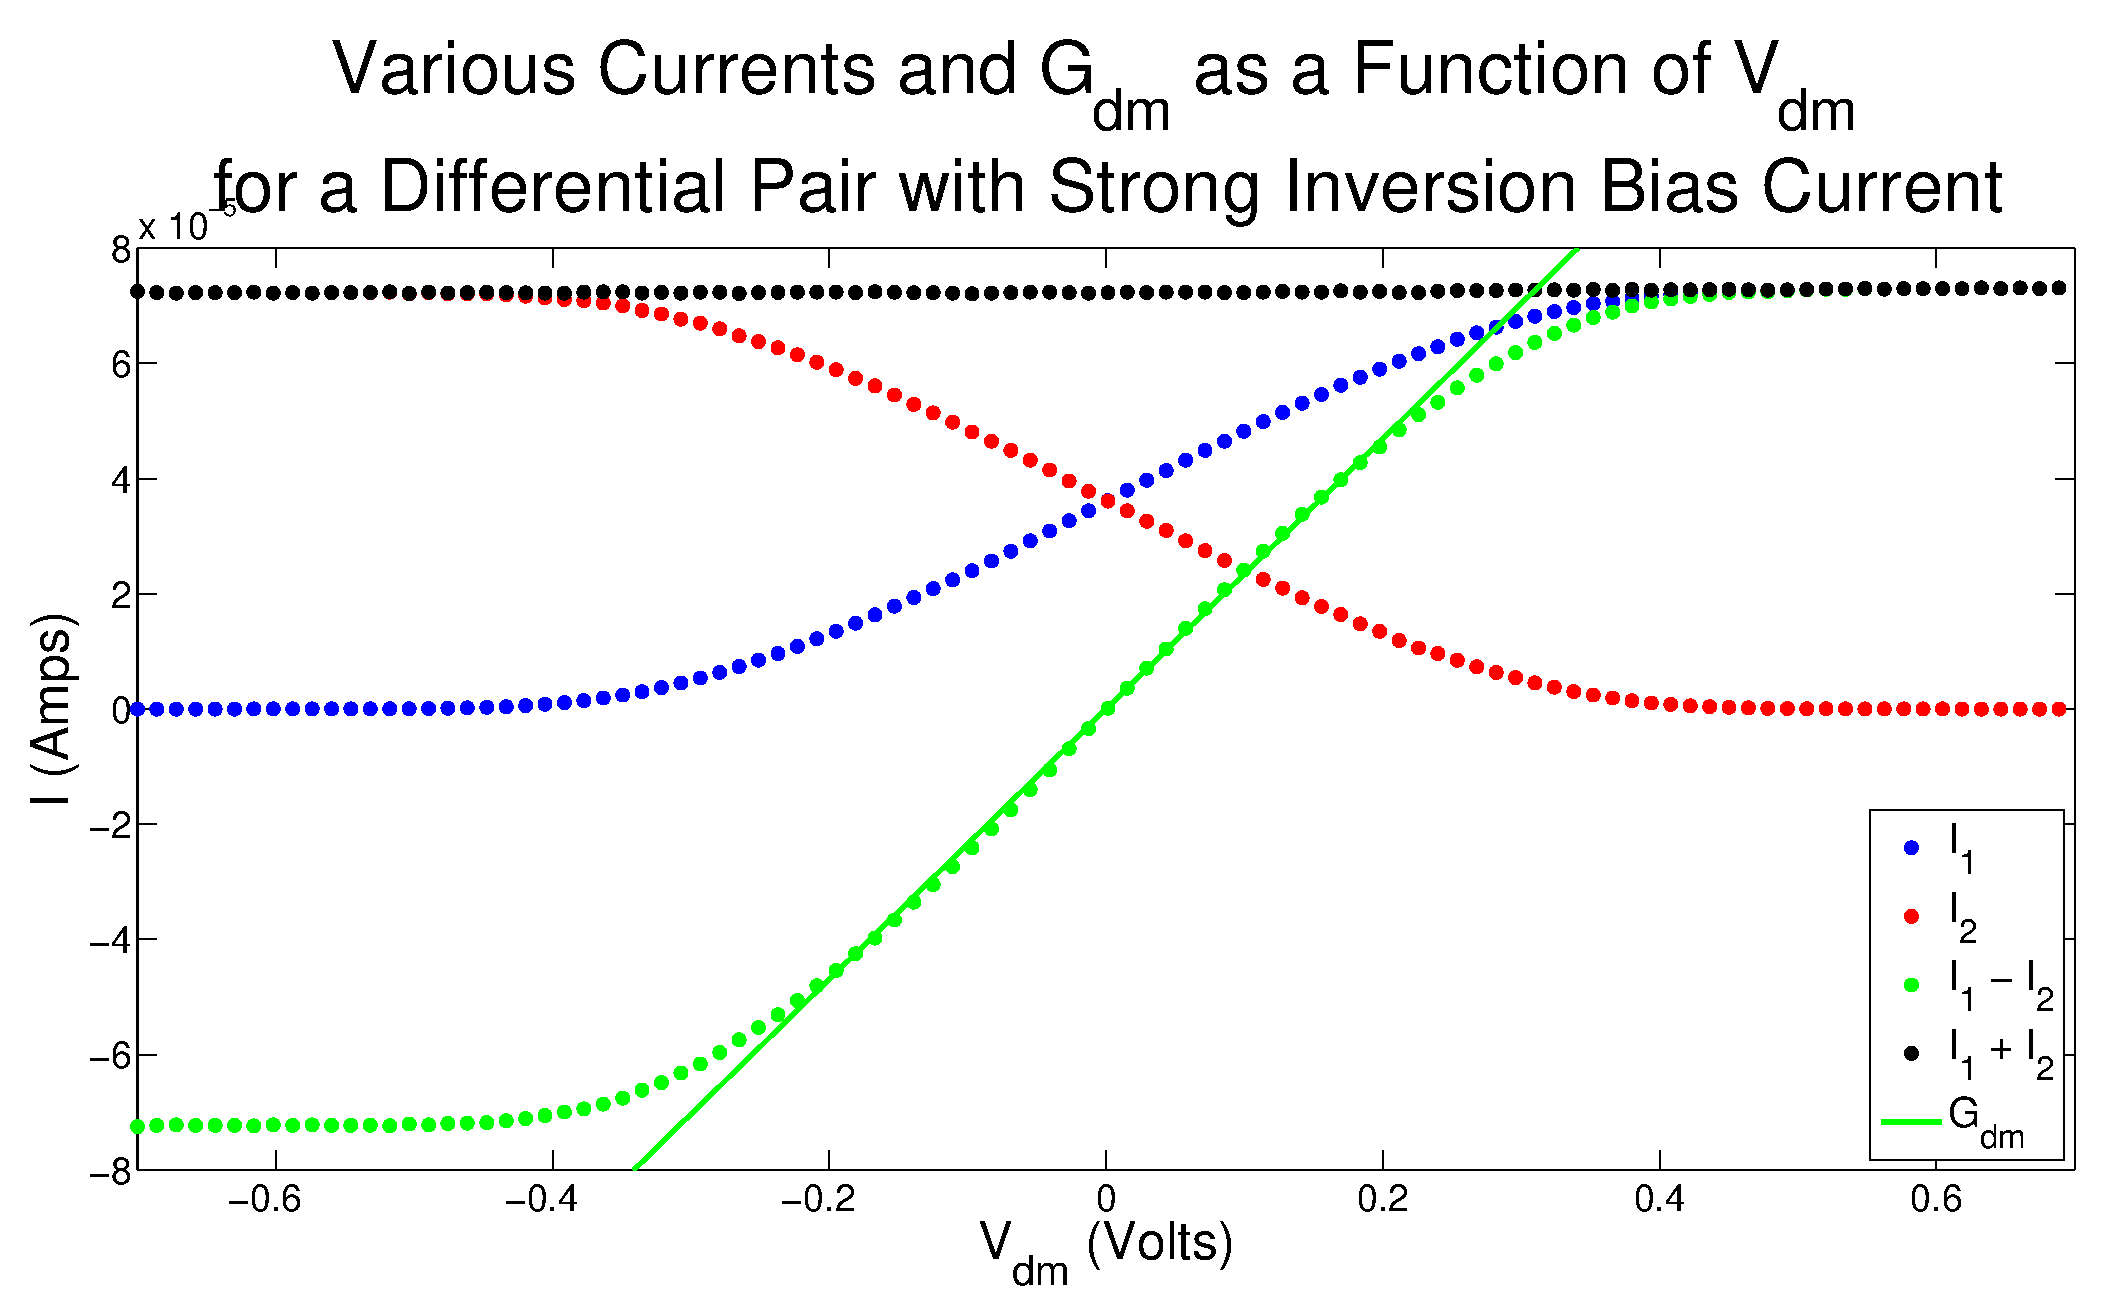
\includegraphics[width=\linewidth]{./Figures/AllCurrentsStrongInversion.eps}
\caption{Something descriptive. }
\label{fig:AllCurrentsStrongInversion }
\end{figure}

%NoldeVoltageStrongInversion

\begin{figure}[H]
\centering
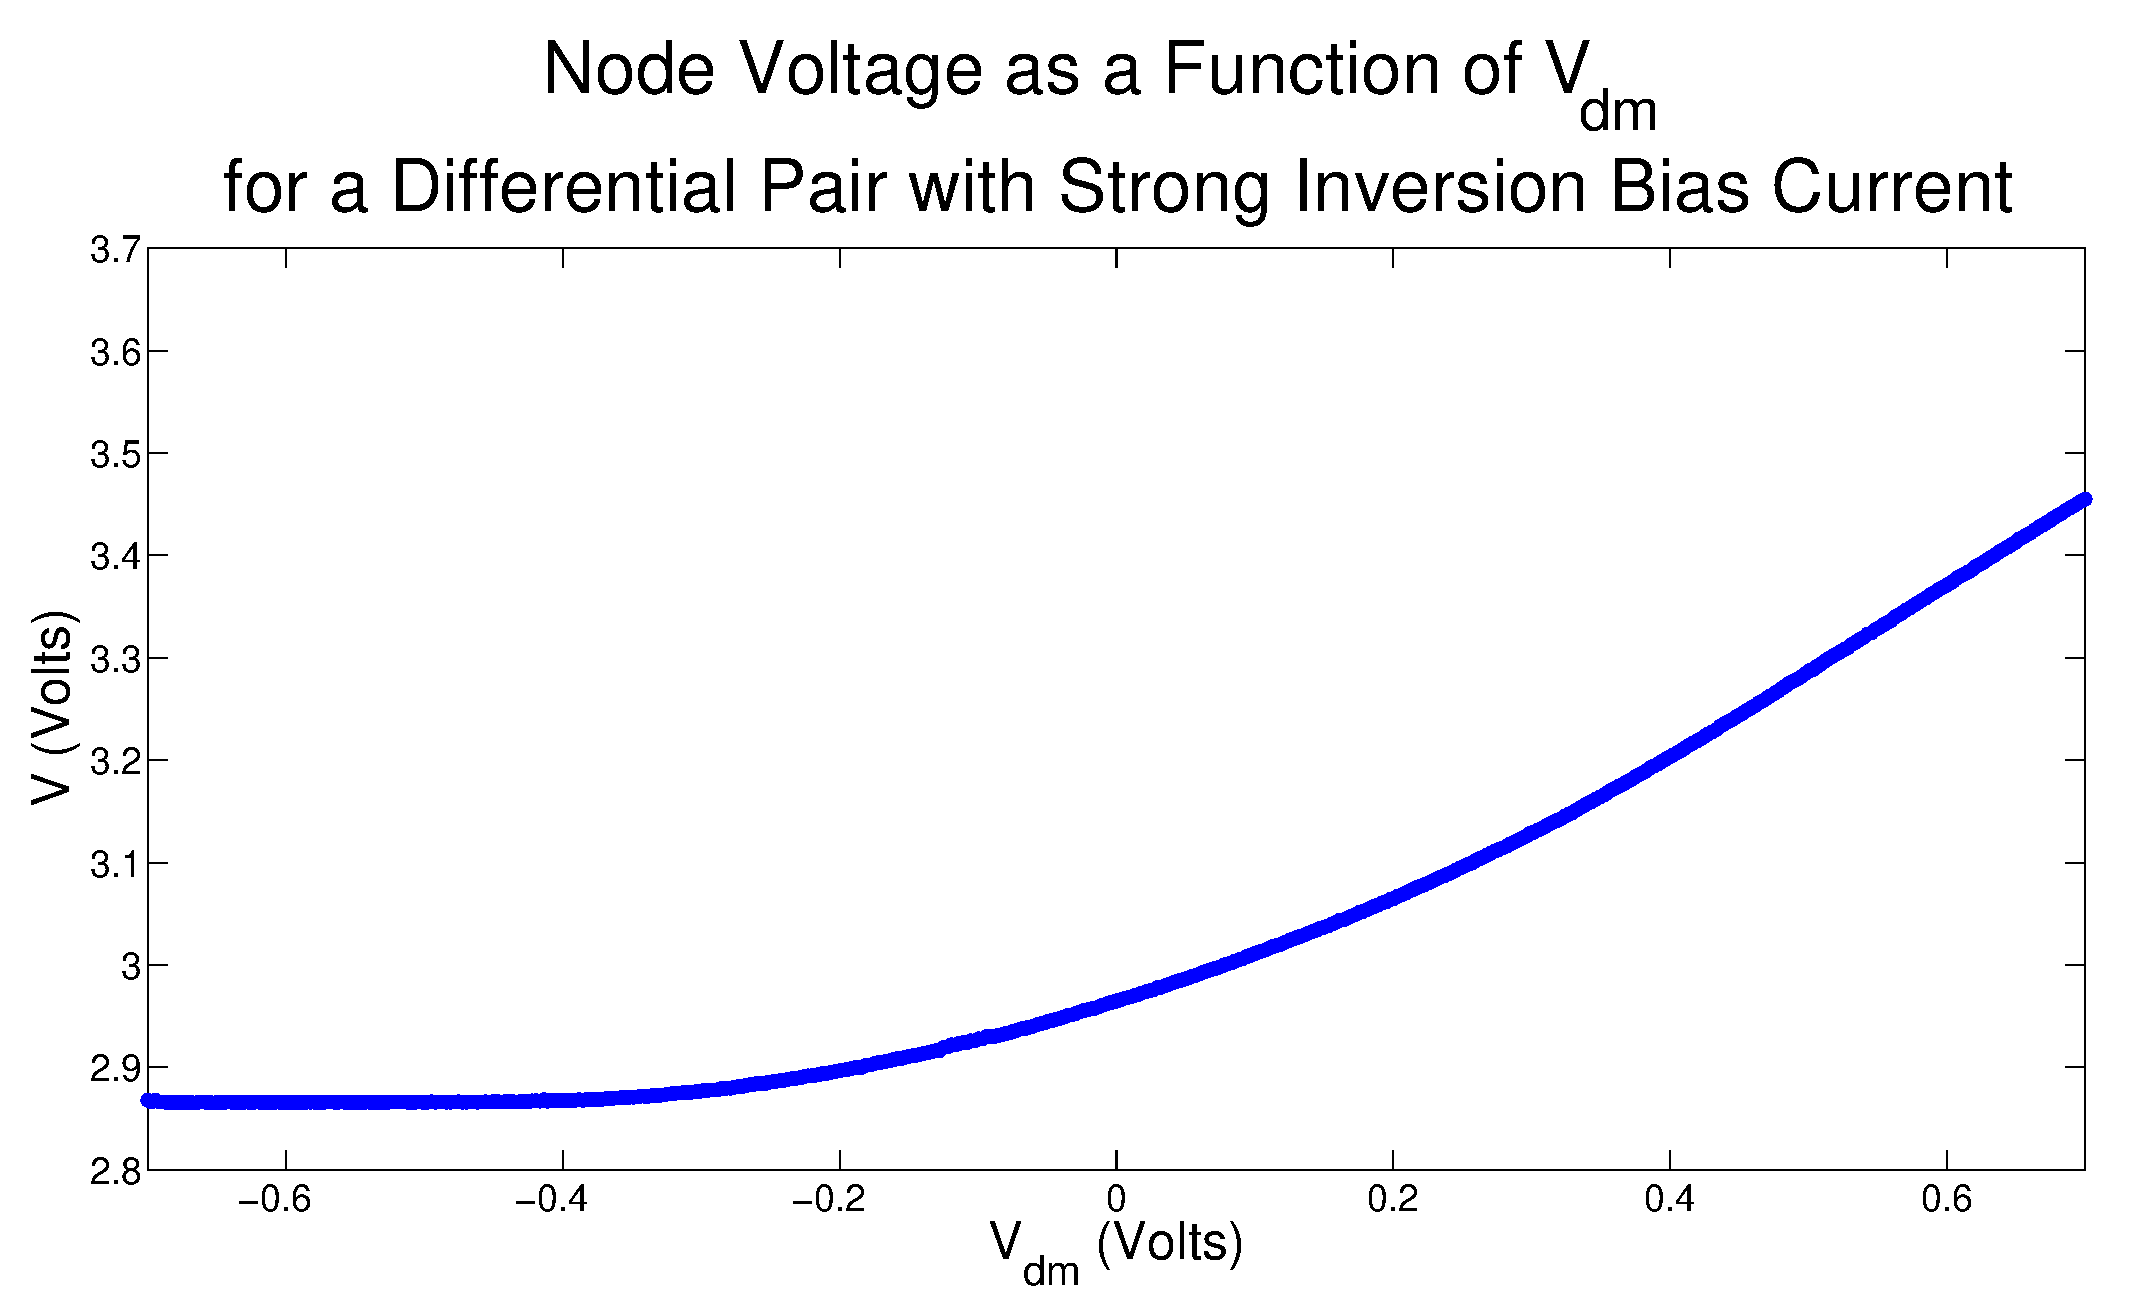
\includegraphics[width=\linewidth]{./Figures/NodeVoltageStrongInversion.eps}
\caption{The node voltage follows the larger voltage!!}
\label{fig:nodevoltageSI}
\end{figure}


\end{document}